\subsection{Explicación formal del problema}

El ejercicio tiene una bella historia detras pero a la hora de pensar el problema resulta útil abastraernos un poco y pensarlo en terminos de objetos matemáticos. Sobre el plano tenemos un conjunto de puntos $ \{ (X_1,Y_1), (X_2,Y_2), (X_3,Y_3),..., (X_n,Y_n) \} $ todos sus elementos cumplen que $X_1 > X_2 > ... > X_n \geq 0 $ y $ 0 \leq Y_1 < Y_2 < .. < Y_n $. O sea están todos repartidos en el primer cuadrante y formando una especie de escalera decreciente de izquierda a derecha. El objetivo es cubrir a todos los puntos con la menor cantidad de rectangulos que cumplan que sus lados son paralelos a los ejes y sus extremos estan en $ (0,0) $ y $ (X_i + T, Y_i + T) $. Donde T es una número entero pasado como parametro y $(X_i,Y_i)$ son las coordenadas de algún punto del conjunto.

Esto se debe resolver en $ O(n)$ y expresar cuales puntos del conjunto se utilizan como extremos de los rectángulos.

Veamos algunos ejemplos de soluciones correctas e incorrectas para terminar de entender lo que plantea el ejercicio. Analicemos el conjunto de puntos $\{(4,2),(3,3),(2,4),(1,5)\}$ y T = 1.

\begin{figure}[H]
\centering
\begin{minipage}{0.49\textwidth}
  \centering
    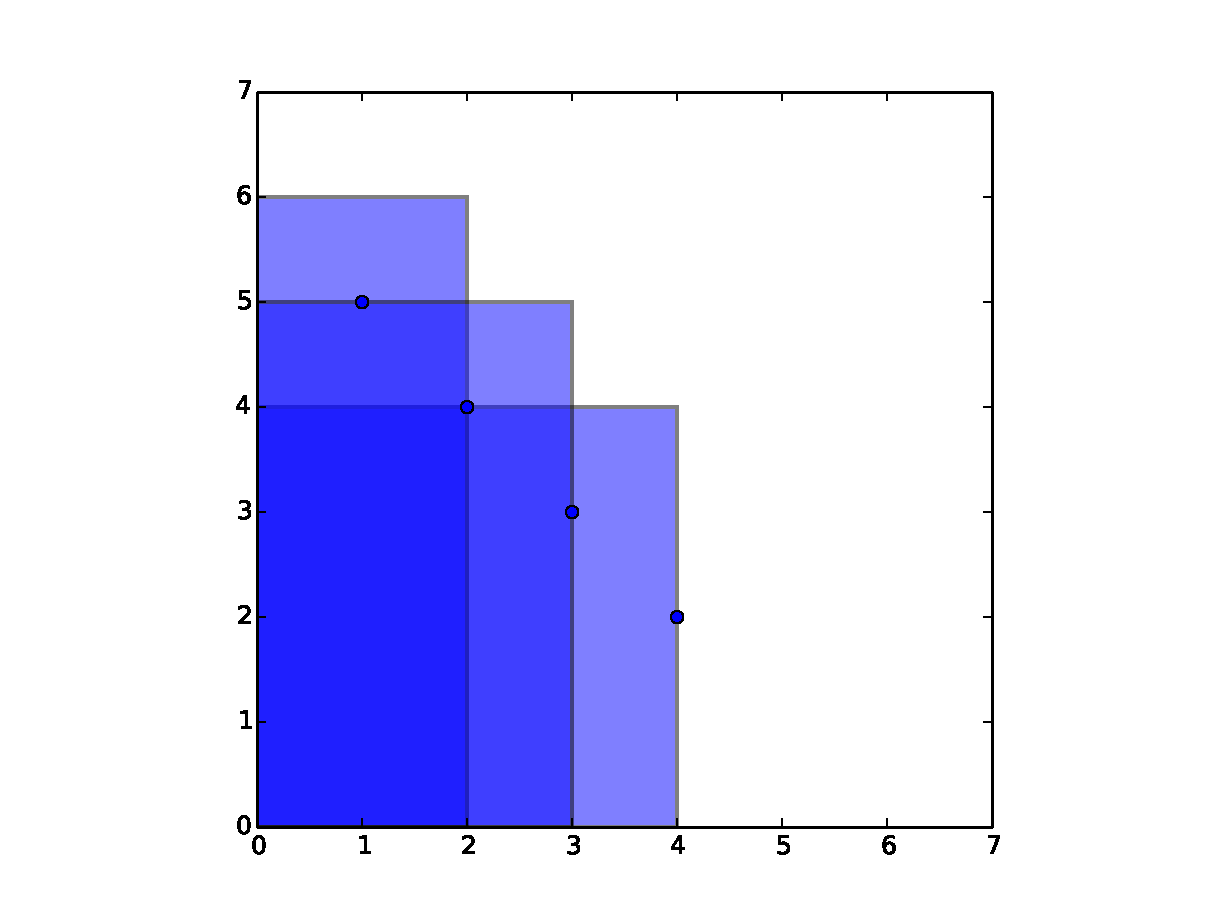
\includegraphics[width=1\textwidth]{img/ejemplos/ej2-1.pdf}
  \caption{\footnotesize Posible elección de rectangulos no óptima.}
  \label{fig:ej3-1}
\end{minipage}%
\hspace{0.01\textwidth}
\begin{minipage}{0.49\textwidth}   
  \centering
    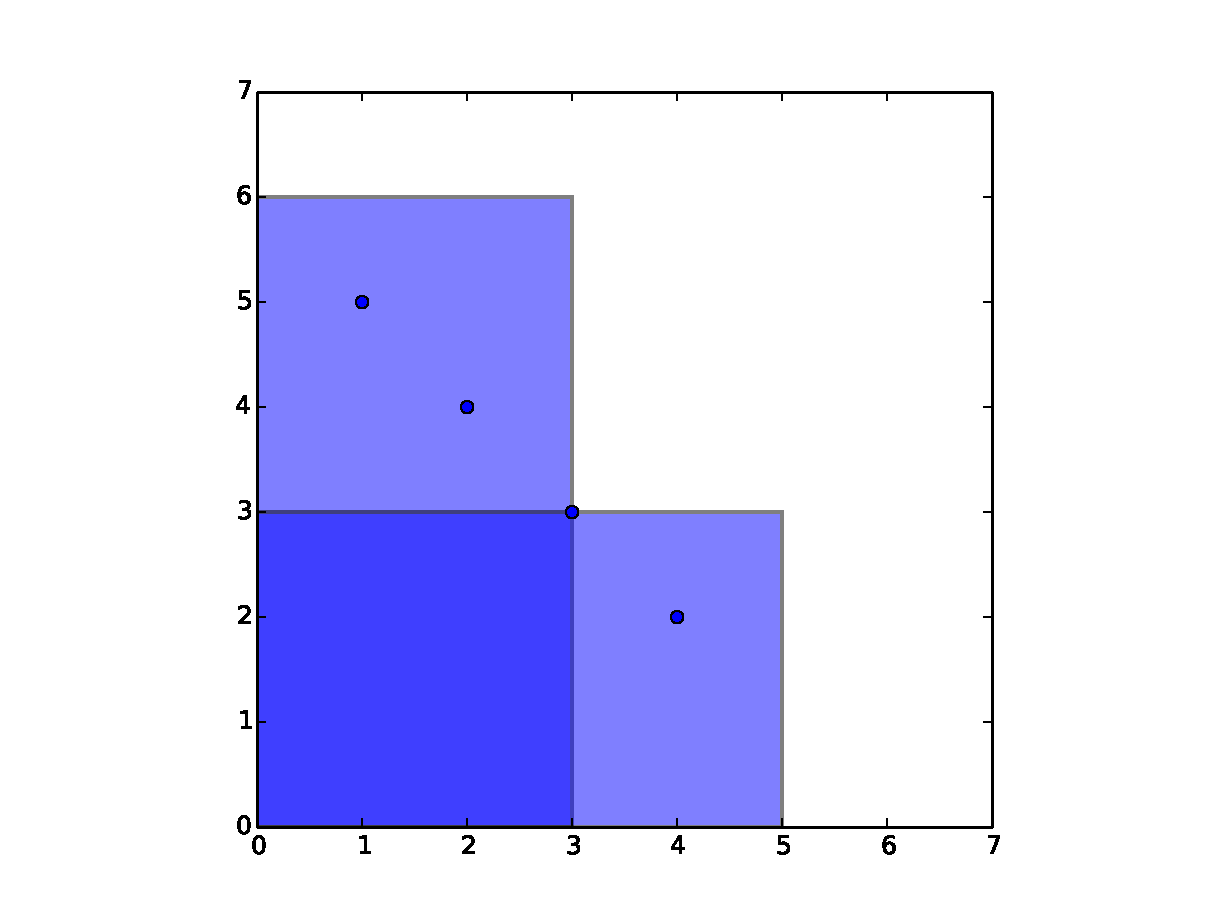
\includegraphics[width=1\textwidth]{img/ejemplos/ej2-2.pdf} 
  \caption{\footnotesize Posible elección de rectangulos incorrecta.}
  \label{fig:ej3-2}
\end{minipage}%
\end{figure}

Algunos ejercicios pueden tener varias soluciones posibles. En este caso tenemos estas dos posibilidades.

\begin{figure}[H]
\centering
\begin{minipage}{0.49\textwidth}
  \centering
    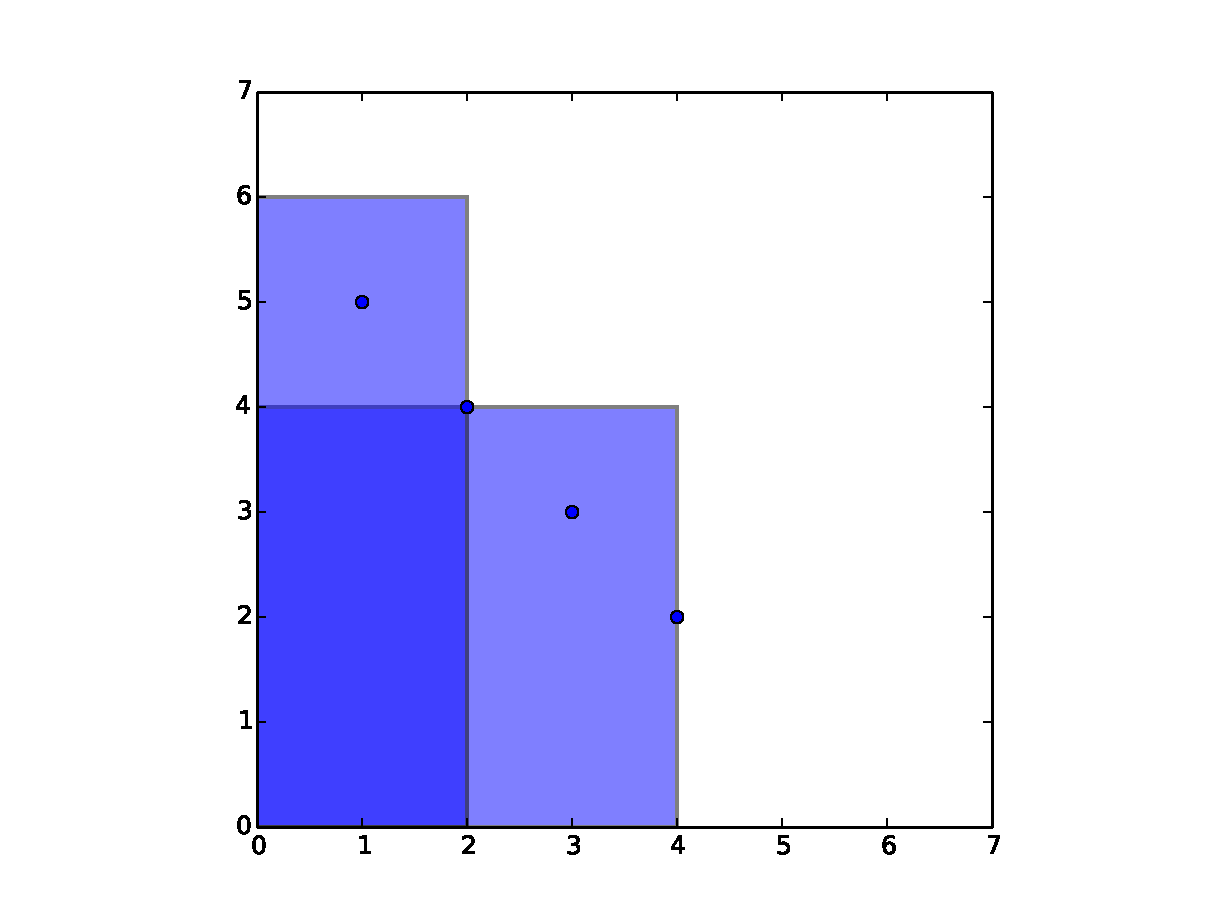
\includegraphics[width=1\textwidth]{img/ejemplos/ej2-3.pdf}
  \caption{\footnotesize Posible elección de rectangulos óptima y correcta.}
  \label{fig:ej3-1}
\end{minipage}%
\hspace{0.01\textwidth}
\begin{minipage}{0.49\textwidth}   
  \centering
    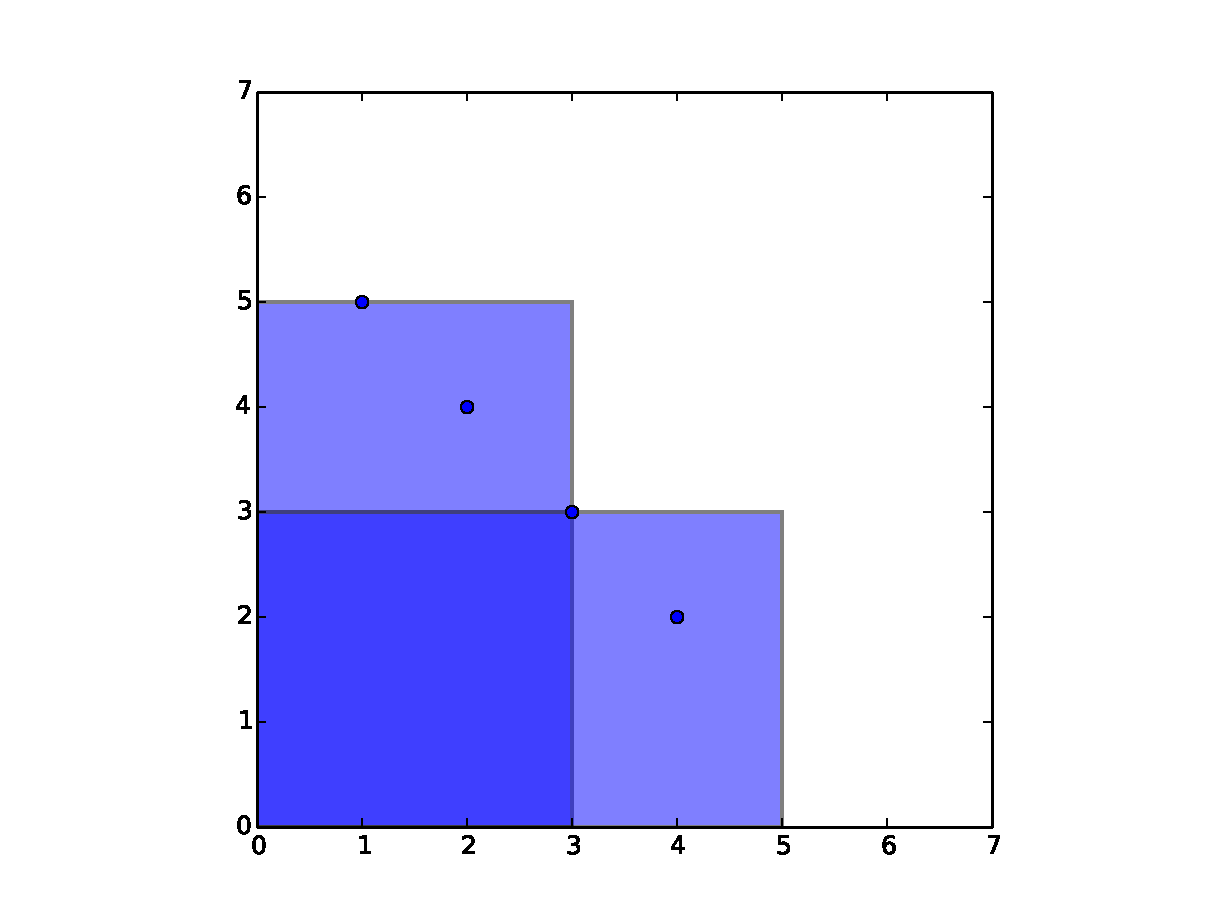
\includegraphics[width=1\textwidth]{img/ejemplos/ej2-4.pdf} 
  \caption{\footnotesize Posible elección de rectangulos óptima y correcta.}
  \label{fig:ej3-2}
\end{minipage}%
\end{figure}


\subsection{Explicación de la solución}

Para resolver el ejercicio utilizamos un $algoritmo$ $goloso$. La idea es ir cubriendo todos los puntos de derecha a izquierda utilizando la menor cantidad de rectangulos posible. La técnica que utilizaremos para lograr esto, la cual veremos luego que es óptima, será por cada iteración del algoritmo buscar un rectángulo que cubra al punto mas a la derecha y al mismo tiempo cubra a la mayor cantidad posible de otros puntos, o sea en cada iteración intentará hacer lo mejor posible para ese momento en particular, por eso lo $greedy$ o $goloso$.

Para la implementación del algoritmo tenemos como datos de entrada los puntos y el valor de $T$, utilizamos una variable $j$ la cual representa el punto mas a la derecha, al cual vamos a cubrir si o si en esa iteración y una variable $i$ la cual representa el candidato a extremo del rectángulo. Comenzamos por el punto mas a la derecha y vamos siguiendo hacia los que tienen una coordenada x menor. Como sabemos que los puntos cumplen que $X_1 > X_2 > ... > X_n \geq 0$ entonces simplemente arrancamos por $X_1$ y seguimos hasta $X_n$, esto se hace facilmente recorriendo el vector $puntos$ desde su posición $0$ hasta $n-1$. El ciclo principal se encarga de buscar en cada iteración el mejor punto para utilizar como extremo de rectángulo y termina cuando j alcanza a n, lo cual implica que ya se cubrieron todos los puntos.

Veamos el pseudocodigo para que termine de quedar claro todo esto.

\begin{algorithm}[H]
\begin{algorithmic}
\caption{Esbozo del algoritmo de Genkidama}
  \Procedure{aQuienDisparo}{vector(int,int) $puntos$, int $t$}
	\State int n = puntos.cantidad()
	\State int i = 0
	\State int j = 0
    \While {$j < n$}
    		\State i = j
		\While { $...$ }
			\State $ i++ $
	  	\EndWhile
		\State $respuesta.agregarA(i)$
		\State $ i++ $
		\While { $ ... $ }
			\State $ j++ $
	 	\EndWhile
  \EndWhile
  \EndProcedure
\end{algorithmic}
\end{algorithm}

Para lograr hacer lo dicho previamente el ciclo principal cuenta con dos bucles anidados.

El primer ciclo tiene como objetivo cubrir a j y al mismo tiempo verificar si no puede cubrir algunos mas. En el pseudocódigo se puede ver facilmente como hacemos eso.

\begin{algorithm}[H]
\begin{algorithmic}

\caption{Ciclo Anidado 1}

\While { $ i < n - 1 \land puntos[i+1].primero + t \geq puntos[j].first $ }
	\State $i++$
\EndWhile

\end{algorithmic}
\end{algorithm}

Si podemos cubrir a un punto mas al mismo tiempo que seguimos cubriendo al punto $(X_i,Y_i)$ entonces guardamos ese nuevo valor como nuestro nuevo candidato para utilizar como extremo del nuevo rectangulo. Repetimos esto hasta que ya consideramos todos los puntos o que el siguiente a nuestro candidato ya no nos permite cubrir a $(X_i,Y_i)$.

Cuando conseguimos al mejor candidato, lo almacenamos y seguimos con el Ciclo Anidado 2.

El segundo ciclo tiene como tarea verificar si al haber agregado el nuevo rectangulo no se cubrieron algunos puntos mas a la izquierda.

\begin{algorithm}[H]
\begin{algorithmic}

\caption{Ciclo Anidado 2}

\While { $ j < n \land puntos[j].segundo \leq puntos[i-1].segundo + T $ }
	\State $j++$
\EndWhile

\end{algorithmic}
\end{algorithm}

En ese caso se aumenta $j$ para que pase a representar al siguiente punto. Se repite esto hasta encontrar uno punto que no haya sido cubierto todavia o hasta que no hayan mas puntos.

\subsubsection{Optimalidad}

Para demostrar que el algoritmo porpuesto es óptimo supondre que no lo es y llegaré a un absurdo. Supongamos que tenemos un algoritmo que si resuelve el problema de manera óptima, tiene que hacer algo distinto a lo que plantea nuestro algoritmo ya que supusimos que no era óptimo. Para diferenciarse del nuestro tiene que tomar al menos una desición distinta.

Dada la solución que suponemos es óptima, nos ponemos a ver las elecciónes de rectangulos que tomó este algoritmo de derecha a izquierda. O sea viendo primero al que tiene como extremo al punto de mayor coordenada x y siguiendo hacia los menores.

Al ponernos a ver elecciones de rectangulos en algun momento vamos a notar que el algoritmo escogió tapar al punto que estaba cubrir mas abajo a la derecha pero sin tapar al mismo tiempo a la mayor cantidad posible de otros puntos sin cubrir. Sabemos que esto va a pasar en algun momento ya que si no fuera asi entonces sería exactamente igual a nuestro algoritmo.

Pero al ver esto se vuelve obvio que esa desición es peor o igual que lo que hacemos, ya que con nuestro algoritmo podriamos reemplazar esa acción por una que cubrá una mayor cantidad de puntos. Terminando en el peor de los casos usando la misma cantidad de rectangulos para la solución. Lo cual es absurdo ya que habiamos supuesto que nuestro algoritmo no era óptimo.



\subsection{Complejidad del algoritmo}

En esta sección demostraremos que el algoritmo tiene una complejidad de $\theta(n)$ donde n es la cantidad de puntos en el plano para cualquier caso (no existe peor ni mejor caso). O sea está acotado inferior y superiormente por n.

Primero se crean variables lo cual cuesta a lo sumo O(n), dependiendo la estructura utilizada, por tener que averiguar la cantidad de puntos en el vector de entrada.

Lo siguiente es el ciclo principal el cual veremos que toma $\theta(n)$. Veamos una serie de proposiciones que utilizaré para demostrarlo, todas son evidentes viendo el pseudocódigo.

\begin{enumerate}

\item Los ciclos 1 y 2 cuestan O(1) por iteración.

\item La variable j aumenta una vez por cada iteracion de cada ciclo en que entra. (En cualquier de los 3 ciclos que hay).

\item Si j vale n entonces terminan todos los ciclos.

\end{enumerate}

Por (3) sabemos que el ciclo solo funcionara mientras j sea menor a n, mientras esto se cumpla se iterara en el ciclo principal y por (1) sabemos que se gastará una cantidad constante de pasos cada vez que se itere en uno de los ciclos internos, por la proposición (2) sabemos que al final de cada iteración del ciclo principal el valor de j será aumentado la cantidad de veces que haya ciclado dentro del primer ciclo anidado mas la cantidad de veces que lo haya hecho en el segundo ciclo anidado mas uno por la iteración principal. Si este valor llega a n el ciclo terminará. Si no ocurre entonces se hará una iteración mas en el ciclo principal. Por lo tanto vamos gastando O(1) cada vez que incrementamos en 1 a j. Y j termina cuando vale n por lo tanto este algoritmo tarda $\theta(n)$, solo nos podemos pasar de ese costo si j llega a valer mas de n y eso no puede pasar por la proposición (3). Tampoco vamos a tardar menos que eso por que eso significaría que j vale menos de n y no puede terminar en ese caso.

Habiendo demostrado esto, sumado a que las instrucciones fuera del ciclo son todas a lo sumo O(n) queda demostrado que la función esta acotada superior e inferiormente por n, para cualquier caso.

\subsection{Performance del algoritmo}

Como vimos anteriormente, el algoritmo tiene una complejidad de $\Theta(n)$. El algoritmo no tiene peor o mejor caso propiamente dichos (dado que es $\Theta(n)$ para todos los casos), pero veremos que las constantes pueden cambiar para algunas entradas por cuestiones de implementación.

\begin{figure}[H]
 \centering
	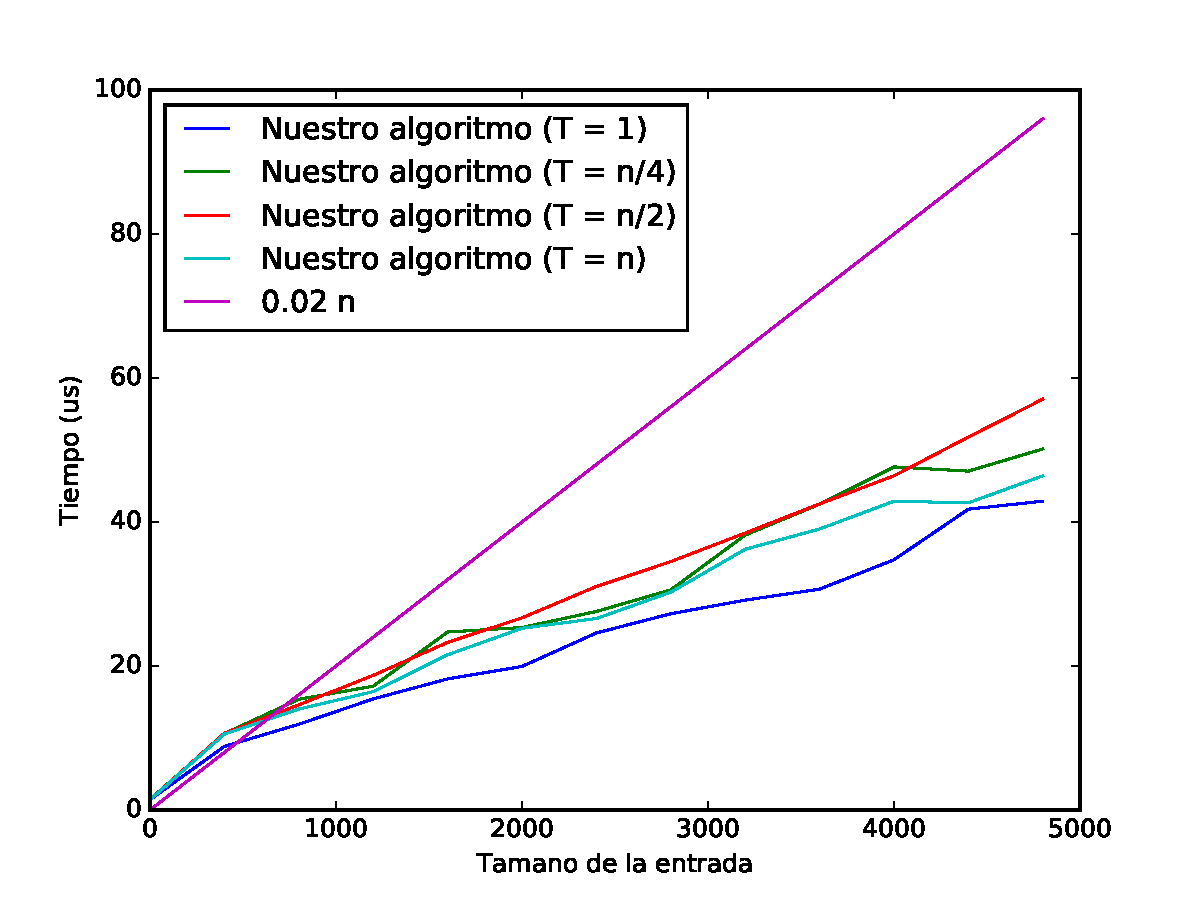
\includegraphics[width=0.8\textwidth]{img/tiempos/genkidama1.pdf}
	\caption{\footnotesize Tiempo que toma el algoritmo en $\mu$s para una entrada de tamaño $n$.}
	\label{fig:genkidama-tiempos1}
\end{figure}

Como se observa, la implementación tiene complejidad lineal, como era esperado. Sin embargo, se observan diferencias según el $T$ que se elija. Recordemos que el $T$ era el radio de impacto del genkidama. Esto se debe a una cuestión de implementacion. Para los casos donde $T = 1$ o $T = n$, nuestra implementación se ahorra entrar a un while, reduciendo la cantidad de instrucciones que ejecuta cada vez.

\begin{figure}[H]
 \centering
	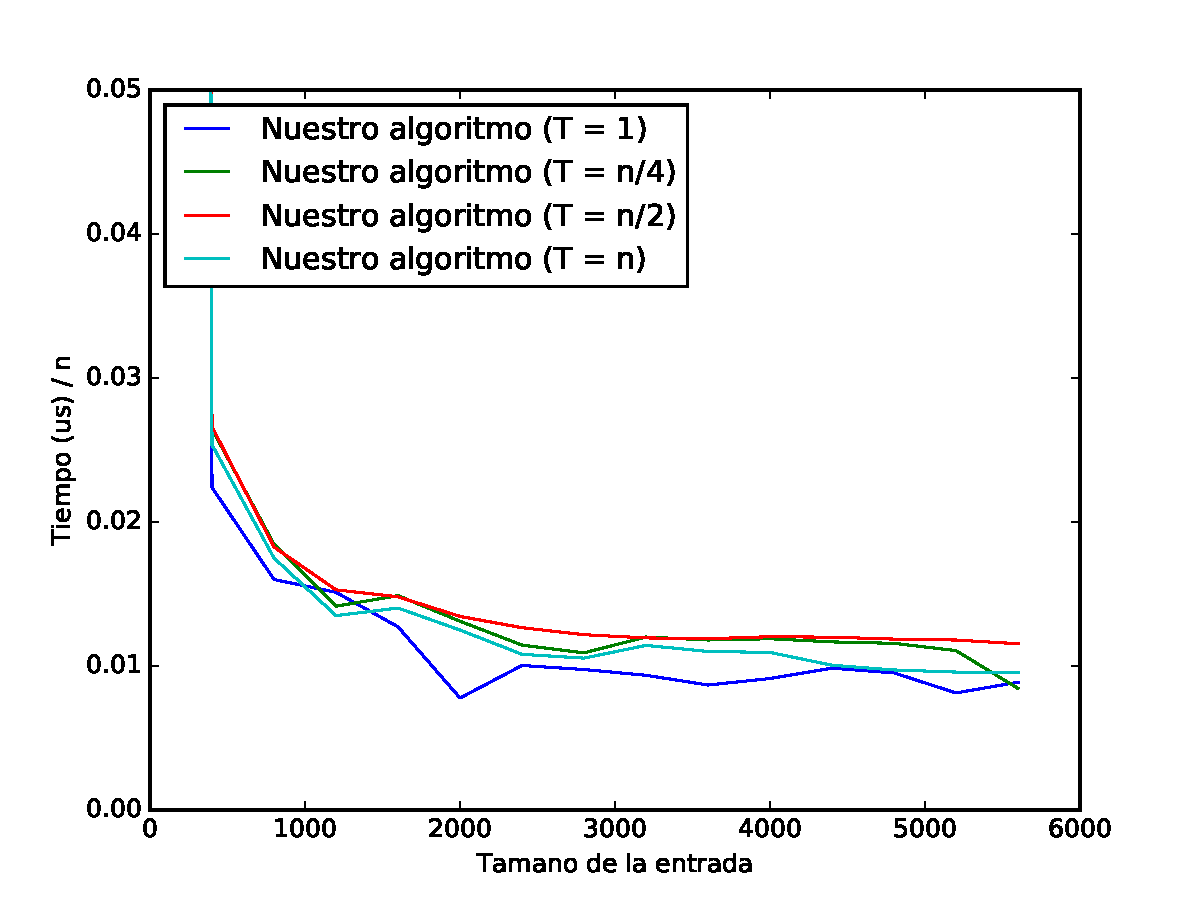
\includegraphics[width=0.8\textwidth]{img/tiempos/genkidama2.pdf}
	\caption{\footnotesize Tiempo que toma el algoritmo en $\mu$s dividido $n$ para una entrada de tamaño $n$.}
	\label{fig:genkidama-tiempos2}
\end{figure}

Este gráfico nos ayuda aún más a confirmar la complejidad lineal de este algoritmo, ayudandonos a ver las constantes para cada caso. Nuevamente, observamos que el caso $T = 1$ tiene una constante un poco menor, debido a lo explicado anteriormente.

Finalmente, veamos que, para instancias de igual tamaño, el tiempo que se tarda en resolverlas no varía demasiado (confirmando el hecho de que para $T$ fijo, la elección de los puntos no cambia el tiempo de ejecución de manera significativa).

\begin{figure}[H]
 \centering
	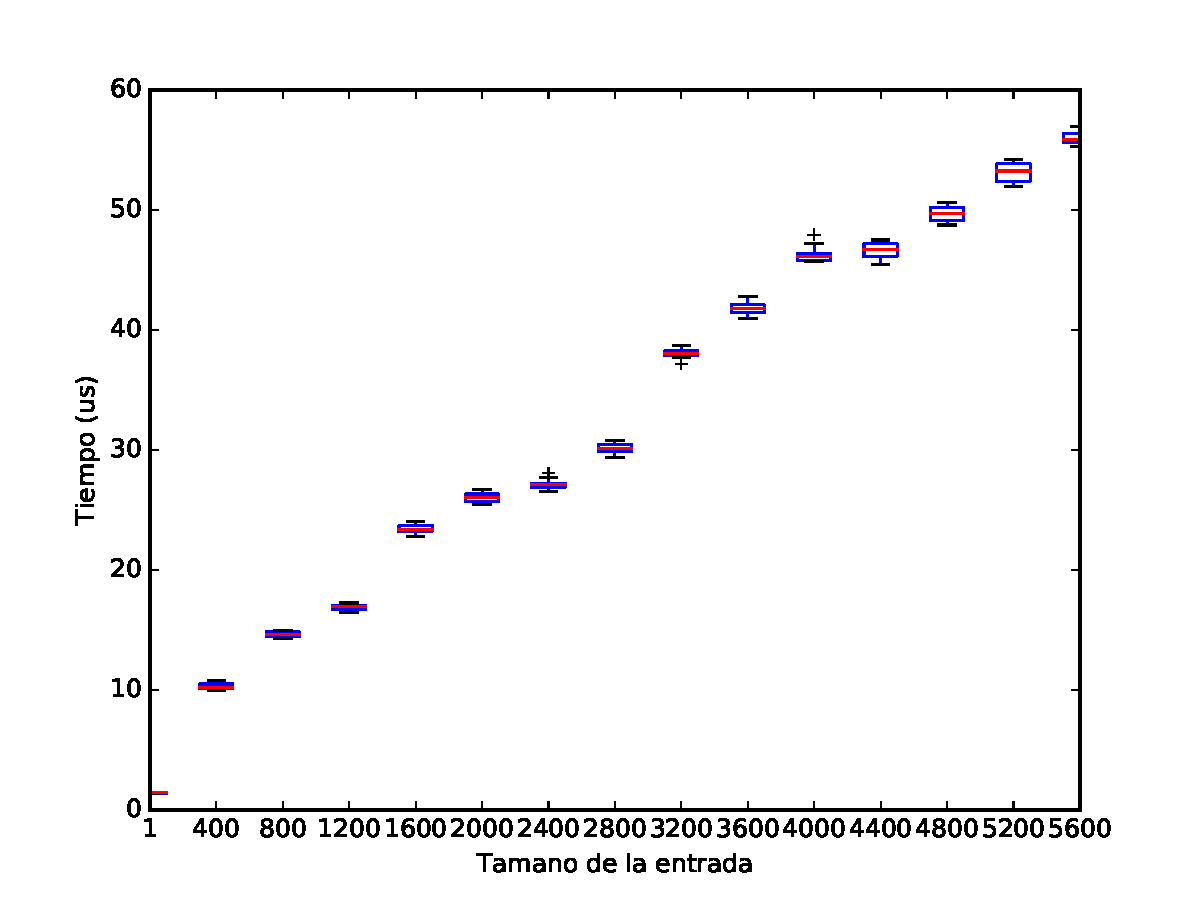
\includegraphics[width=0.8\textwidth]{img/tiempos/genkidama3.pdf}
	\caption{\footnotesize Tiempo que toma el algoritmo en $\mu$s para una entrada de tamaño $n$. $T = n/4$. Se indican los valores del primer al tercer cuatril con un rectángulo azul y la mediana con una linea roja. El máximo y minimo se indican con lineas negras arriba y abajo del rectángulo.}
	\label{fig:genkidama-tiempos3}
\end{figure}

\subsubsection{M\'etodo de experimentación}

Para los primeros dos gráficos (es decir, para la figura \label{fig:genkidama-tiempos1} y la figura \label{fig:genkidama-tiempos2}), generamos 50 instancias al azar de para cada $n$.
Las instancias fueron generadas de la siguiente manera: para cada $n$, elegimos $n$ puntos al azar de la grilla $\{1,..., n^2\} \times \{1, ... , n^2\}$.
Estos puntos eran elegidos al azar usando el mismo \emph{seed} cada vez (para la instancia 1 usabamos 1 como seed, para la instancia 2, usabamos 2, etc.), de tal manera que los experimentos fueran reproducibles de una manera válida.

Cada instancia fue ejecutada 20 veces, y el resultado final era el mínimo de todas las corridas.
Luego, tomabamos la mediana de todas las instancias.
Es decir, el restultado final es la mediana de los mínimos. Como puede observarse en la figura \ref{fig:genkidama-tiempos3}, la mediana es muy representativa de lo que sucede.
